% Tsunagu: technical report.
% Build from this folder: latexmk -pdf tsunagu.tex
% Every result number is \input from results/*.tex, which `tsunagu report` generates
% from the same data as results/results.md. Do not type result numbers in this file.
\documentclass[11pt,a4paper]{article}

\usepackage[T1]{fontenc}
\usepackage[utf8]{inputenc}
\usepackage{lmodern}
\usepackage{microtype}
\usepackage[margin=2.3cm]{geometry}
\usepackage{amsmath}
\usepackage{booktabs}
\usepackage{enumitem}
\usepackage{xcolor}
\usepackage{listings}
\usepackage{caption}
\usepackage{tikz}
\usetikzlibrary{arrows.meta,positioning}
\usepackage[hidelinks]{hyperref}

\definecolor{codebg}{gray}{0.96}
\definecolor{pending}{rgb}{0.75,0.1,0.1}
\lstset{
  basicstyle=\ttfamily\footnotesize,
  backgroundcolor=\color{codebg},
  breaklines=true,
  columns=fullflexible,
  frame=single,
  rulecolor=\color{gray!40},
  showstringspaces=false,
}
\newcommand{\code}[1]{\texttt{#1}}
\newcommand{\owner}[1]{\noindent\textcolor{pending}{\textit{[To be written by the owner: #1]}}}
\setlist{itemsep=2pt,topsep=4pt}

\title{Tsunagu: GraphRAG versus vector RAG\\on cross-referenced technical documentation}
\author{Fay\c{c}al Raghibi}
\date{22 October 2026}

\begin{document}
\maketitle
\sloppy

\begin{abstract}
Tsunagu (\emph{to connect}) is a one-day personal prototype that asks whether a graph layer
(explicit page links, code symbols and relations extracted by a language model) improves
answers to relational, multi-hop and enumerative questions over a heavily cross-referenced
technical documentation, compared with a dense vector RAG and a cheap hybrid RAG (BM25 and
dense retrieval fused with reciprocal rank fusion), and at what cost. The corpus is the
LangGraph documentation pinned at one commit. All three systems share the same chunks, the
same answering model, the same prompt and the same top-$k$ budget, so the retriever is the
only variable. This report describes the project structure, every component, the experimental
protocol and the results. Result numbers are not typed by hand: they are generated by
\code{tsunagu report} and included verbatim.
\end{abstract}

\tableofcontents
\newpage

%=====================================================================
\section{Status of this document}
%=====================================================================

\begin{itemize}
  \item \textbf{Done:} corpus, ingestion, dense and hybrid indexes, graph construction and
  entity resolution, merge review, retrieval-only evaluation, full evaluation (30 questions,
  3 systems, 3 repeats, 270 answered and judged rows, no parse failure).
  \item \textbf{Pending:} judge calibration (human gate G3). Twenty blind items in
  \code{data/labels\_manual.csv} wait for the owner's scores. Until they exist, every
  correctness number in Section~\ref{sec:results} comes from an LLM judge whose agreement
  with a human is \emph{not measured yet}. The calibration line in the results says so.
  \item \textbf{Owner sections:} Findings, Limits and ``What I would do at Safran''
  (Sections~\ref{sec:findings} to \ref{sec:safran}) are written by the owner only.
\end{itemize}

To refresh the numbers after calibration: run \code{tsunagu calib}, then \code{tsunagu report},
then rebuild this PDF.

%=====================================================================
\section{Research question}
%=====================================================================

\paragraph{Question.} On a corpus of technical documentation full of cross-references, does a
graph layer (entities, relations, explicit links between pages) improve answers to relational,
multi-hop and enumerative questions, compared with (1) a dense vector RAG and (2) a hybrid RAG
(BM25 plus dense, fused with reciprocal rank fusion)? And what does it cost in indexing tokens,
indexing time, query latency and entity-resolution effort?

\paragraph{Why a hybrid control.} Many published ``GraphRAG wins'' are really ``anything beats
naive dense retrieval'' wins. A lexical-plus-dense hybrid is cheap and strong on exact
identifiers. Comparing the graph with the hybrid, not only with dense, separates the value of
the \emph{graph} from the value of \emph{better retrieval in general}.

\paragraph{Why this corpus.} The LangGraph documentation has the properties of industrial
technical documentation, which motivates the comparison:

\begin{center}
\begin{tabular}{ll}
\toprule
LangGraph docs & Industrial technical documentation \\
\midrule
Links between pages & References between documents \\
API symbols (\code{StateGraph}, \code{InMemorySaver}) & Exact references: part numbers, document ids \\
Deprecated APIs, version notes & Revisions, applicability by version \\
``Feature X requires Y'' & ``Procedure X applies under condition Y'' \\
\bottomrule
\end{tabular}
\end{center}

%=====================================================================
\section{Provenance and honesty contract}
%=====================================================================

The project follows a written honesty contract (\code{docs/graphrag\_prototype\_spec.md},
Section~0). Its rules, and the places where reality differed from the plan:

\begin{enumerate}
  \item \textbf{Numbers.} Every result number comes from \code{results/results.md}, generated
  by \code{tsunagu report}. This document includes the same numbers through
  \code{results/results\_auto.tex} and \code{results/observations.tex}, which the same command
  writes by converting the same Markdown. Nothing is transcribed by hand.
  \item \textbf{Question set and merge labels.} The plan had the owner writing the 30 questions
  and labelling the merge review. On 22 October 2026 the owner asked the AI assistant to do
  both. They were written from the cleaned corpus \emph{before any retrieval or answer result
  existed}, and the question file was hashed (\code{results/questions\_lock.json}) before the
  first run. Consequences, recorded in the design addendum (fact 5): the question set may
  favour structures the graph handles well, because the same assistant designed the graph
  retriever; the false-merge rate reflects the assistant's judgement, not a human one.
  \item \textbf{Judge calibration stays human.} \code{data/labels\_manual.csv} is owner-only:
  a model labelling answers to calibrate a model judge would defeat its purpose.
  \item \textbf{One revision after seeing results.} The graph retriever was revised once after
  the first retrieval-only run, because it had collapsed into dense retrieval
  (Section~\ref{sec:graph-retriever}). This is a stated limit.
  \item \textbf{Conclusions.} Findings, Limits and the Safran section are the owner's.
\end{enumerate}

%=====================================================================
\section{Project structure}
%=====================================================================

\subsection{Pipeline}

\begin{center}
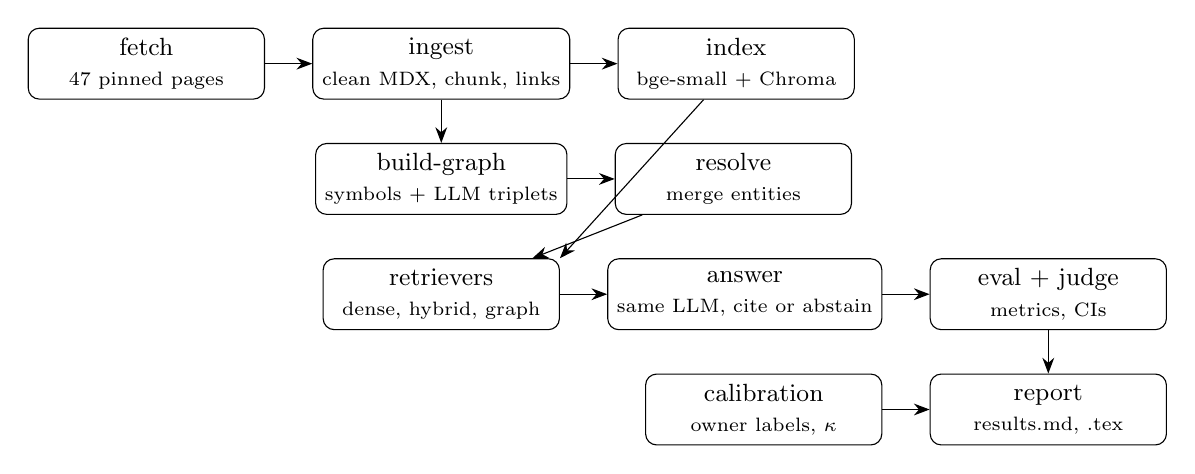
\begin{tikzpicture}[
  box/.style={draw, rounded corners, align=center, font=\small, minimum width=3.0cm, minimum height=0.9cm},
  arr/.style={-{Stealth[length=2mm]}},
  node distance=0.55cm and 0.6cm]
\node[box] (fetch) {fetch\\\scriptsize 47 pinned pages};
\node[box, right=of fetch] (ingest) {ingest\\\scriptsize clean MDX, chunk, links};
\node[box, right=of ingest] (index) {index\\\scriptsize bge-small + Chroma};
\node[box, below=of ingest] (graph) {build-graph\\\scriptsize symbols + LLM triplets};
\node[box, right=of graph] (resolve) {resolve\\\scriptsize merge entities};
\node[box, below=of graph] (retr) {retrievers\\\scriptsize dense, hybrid, graph};
\node[box, right=of retr] (answer) {answer\\\scriptsize same LLM, cite or abstain};
\node[box, right=of answer] (eval) {eval + judge\\\scriptsize metrics, CIs};
\node[box, below=of eval] (report) {report\\\scriptsize results.md, .tex};
\node[box, left=of report] (calib) {calibration\\\scriptsize owner labels, $\kappa$};
\draw[arr] (fetch) -- (ingest);
\draw[arr] (ingest) -- (index);
\draw[arr] (ingest) -- (graph);
\draw[arr] (graph) -- (resolve);
\draw[arr] (index) -- (retr.north east);
\draw[arr] (resolve) -- (retr);
\draw[arr] (retr) -- (answer);
\draw[arr] (answer) -- (eval);
\draw[arr] (eval) -- (report);
\draw[arr] (calib) -- (report);
\end{tikzpicture}
\end{center}

Each box is a \code{tsunagu} command (Typer CLI). Every LLM call goes through one cached client,
so re-running any stage costs nothing once its calls are cached.

\subsection{Repository layout}

\begin{center}
\small
\begin{tabular}{p{4.6cm}p{10.4cm}}
\toprule
Path & Role \\
\midrule
\code{config.yaml} & Single source of settings: page list, LLM, chunking, retrieval, graph, evaluation. \\
\code{aliases.yaml} & Hand-written alias map for entity resolution (canonical name: aliases). \\
\code{src/tsunagu/config.py} & Pydantic models for \code{config.yaml}. \\
\code{corpus.py} & Downloads the 47 pages at the pinned commit. \\
\code{mdx.py} & Turns Mintlify MDX into plain Markdown, Python variant only. \\
\code{links.py} & Normalises internal links to page ids. \\
\code{chunking.py} & Heading-aware chunker that never splits a code block; symbol extraction. \\
\code{ingest.py} & Writes chunks, link edges, corpus statistics and a page index. \\
\code{tokens.py} & cl100k token counting. \\
\code{llm.py} & OpenAI-compatible client for NVIDIA NIM: disk cache, rate limit, retries, usage log. \\
\code{embeddings.py}, \code{store.py} & bge-small embedder; in-memory chunk store. \\
\code{vector\_index.py}, \code{index.py} & ChromaDB dense index and saved embedding matrices. \\
\code{retrievers.py} & Dense, BM25 and hybrid (RRF) retrievers. \\
\code{extract.py} & Schema-guided triplet extraction (LlamaIndex backend and JSON backend). \\
\code{graph.py} & JSON property graph: nodes, edges, provenance, statistics. \\
\code{resolve.py} & Entity resolution, merge log, random merge review sample. \\
\code{graph\_retriever.py} & Graph retriever: seeds, expansion, ranking. \\
\code{systems.py} & Builds the three systems from config. \\
\code{answer.py} & Shared answering prompt, JSON parsing, one retry, abstention. \\
\code{judge.py} & Correctness, faithfulness and citation-precision judges. \\
\code{questions.py} & Question model and validator. \\
\code{metrics.py} & hit@k, recall@k, MRR, Wilson interval, Cohen's $\kappa$, percentiles. \\
\code{runner.py} & Runs retrieval, answering and judging for every question and system. \\
\code{calibration.py} & Blind label sample and judge-versus-human agreement. \\
\code{report.py} & Generates the tables, observations and their LaTeX copies. \\
\code{cli.py} & Typer commands. \\
\code{tests/} & 22 test modules, 102 tests, run offline with fake LLMs and embedders. \\
\code{data/} & Raw corpus, processed chunks, graph files, questions, manual labels. \\
\code{index/} & Chroma database and embedding matrices. \\
\code{results/} & Every generated artefact: rows, logs, merge review, calibration, report. \\
\code{cache/llm/} & One file per LLM call, keyed by its full request. \\
\code{docs/} & Spec, design addendum, implementation plan, this report. \\
\bottomrule
\end{tabular}
\end{center}

\subsection{Engineering conventions}

Python~3.12 in a dedicated virtual environment; type hints and
\code{from \_\_future\_\_ import annotations} everywhere; Google docstrings. Each behaviour was
written test first. \code{ruff check}, \code{ruff format}, \code{mypy} and \code{pytest} run
before every commit through pre-commit, and again in GitHub Actions. Work happens on the
\code{feat/mvp} branch with Conventional Commits; merging to \code{main} needs the owner's
explicit approval.

%=====================================================================
\section{Corpus and ingestion}
%=====================================================================

\subsection{Source}

The LangGraph documentation moved from \code{langchain-ai/langgraph} to
\code{langchain-ai/docs} and is now written in Mintlify MDX. The corpus is pinned at commit
\begin{center}\code{23152b1133e7759381661e93bcdca778101a80bc}.\end{center}
It contains all of \code{src/oss/langgraph/}
except two changelog stubs and the case studies, plus the concept pages on memory,
human-in-the-loop and context, and the LangChain pages on human-in-the-loop and multi-agent
systems (multi-agent moved to the LangChain section). That gives 47 pages; the exact list is in
\code{config.yaml}. Size and chunk counts appear in the first line of the results.

\subsection{Cleaning MDX}

\code{mdx.py} turns each page into plain Markdown:
\begin{itemize}
  \item front matter is dropped (the title is kept), as are \code{\{/* */\}} comments, snippet
  imports and lines that are only JSX tags (\code{<Note>}, \code{<Tabs>}, \code{<Accordion>});
  \item \code{:::python} blocks are unwrapped and \code{:::js} blocks removed, so the corpus is
  not duplicated in TypeScript;
  \item API references written \code{@[`StateGraph`]} become code spans. They are a free and
  precise symbol signal;
  \item code fences are copied unchanged.
\end{itemize}
Internal links are absolute (\code{/oss/langgraph/persistence}, sometimes
\code{/oss/python/langgraph/...}); \code{links.py} normalises them to page ids such as
\code{langgraph/persistence}. Links that leave the corpus are counted but not kept as edges.

\subsection{Chunking}

Pages are split on headings outside code. Inside a section, paragraphs and whole code blocks are
packed greedily up to 500 tokens (cl100k), with about 50 tokens of trailing prose carried over as
overlap; a block is only split if it is larger than 900 tokens, and code blocks are never cut
mid-block unless they exceed that limit. Each chunk keeps its heading path; its citation label
is \code{page\#last heading}. Symbols are collected from prose code spans and from
\code{from x import A, B} lines in code.

%=====================================================================
\section{The three systems}
%=====================================================================

All three retrieve $k=8$ chunks from the same 732-chunk store and pass them to the same answering
prompt.

\subsection{A. Dense}

Chunks are embedded with \code{BAAI/bge-small-en-v1.5} (384 dimensions, normalised) and stored
in ChromaDB. A query is embedded with the model's query instruction and the 8 chunks with the
highest cosine similarity are returned.

\subsection{B. Hybrid (BM25 + dense, RRF)}

BM25 runs over a tokeniser that lowercases words and also splits camelCase and snake\_case
identifiers, so \code{InMemorySaver} matches ``in memory saver''. Each retriever returns 20
candidates, fused with reciprocal rank fusion:
\[
  \mathrm{RRF}(d) = \sum_{r \in \{\text{bm25},\,\text{dense}\}} \frac{1}{k_{\text{rrf}} + \mathrm{rank}_r(d)},
  \qquad k_{\text{rrf}} = 60,
\]
with ranks starting at 1. The top 8 fused chunks are returned.

\subsection{C. Graph}

\subsubsection{Graph construction}

The graph is a JSON property graph (\code{data/graph/*.json}), chosen over a library store
because one file can be read, diffed and traversed by hand.

\paragraph{Deterministic layer (free).} One \code{Page} node per page; \code{LINKS\_TO} edges from
the normalised links; one \code{Symbol} node per code symbol, with \code{Page -MENTIONS-> Symbol}
edges. Every node stores the ids of the chunks where it appears (\code{chunk\_ids}), which is how
traversal gets back to text.

\paragraph{LLM layer.} Each chunk is sent to the extraction model with a fixed schema:
\begin{itemize}
  \item entity types \code{Concept}, \code{Class}, \code{Function}, \code{Parameter},
  \code{Feature};
  \item relation types \code{USES}, \code{REQUIRES}, \code{CONFIGURES}, \code{PART\_OF},
  \code{ALTERNATIVE\_TO}, \code{DEPRECATED\_BY}, \code{RETURNS};
  \item at most 10 triplets per chunk; names copied as written.
\end{itemize}
A strict filter drops anything outside the schema, empty names and self-loops.

\paragraph{Extraction backend: a measured choice.} The plan was LlamaIndex
\code{SchemaLLMPathExtractor}, with our own JSON prompt as fallback, decided by a 10-chunk spike.
On the real model, LlamaIndex returned 0 triplets on all 10 chunks \emph{without raising any
error}, while the JSON extractor returned triplets on 9 of 10
(\code{results/extraction\_spike.json}). The JSON backend was used for the whole graph. The
lesson: a framework that swallows extraction errors needs a measured check before it is trusted.

\subsubsection{Entity resolution}

Duplicates are merged with a union-find, in four steps; \code{Page} nodes are never touched:
\begin{enumerate}
  \item \textbf{normalize}: same type and same normalised name (lowercase, no backticks or
  \code{()}, separators collapsed, last word singularised);
  \item \textbf{alias}: same canonical name after the hand-written \code{aliases.yaml};
  \item \textbf{symbol\_link}: a deterministic \code{Symbol} joins the LLM code entity
  (\code{Class}, \code{Function}, \code{Parameter}) with the same name. This is the bridge between
  the free skeleton and the LLM layer;
  \item \textbf{embedding}: within a type, entity names whose bge-small cosine similarity is
  above 0.92 are merged, most similar pairs first.
\end{enumerate}
Every union is logged in \code{results/merges.csv}. To estimate the false-merge rate without
bias, 30 embedding merges are drawn at random (seed 42) into \code{results/merges\_review.csv}
and labelled correct or false. Counts per step and the false-merge count are in the ``Graph''
line of the results.

\subsubsection{Graph retriever}
\label{sec:graph-retriever}

\begin{enumerate}
  \item \textbf{Seeds.} Query terms are code spans plus word 1- to 3-grams (stopwords and words
  under 3 characters dropped), normalised like entity names. Any entity whose name or alias
  matches is a seed. In addition, the 5 entities whose name embedding is closest to the query
  become seeds if their similarity is at least 0.6.
  \item \textbf{Expansion.} Breadth-first, 2 hops, over all relations (\code{LINKS\_TO},
  \code{MENTIONS} and the LLM relations). From each node at most 40 neighbours are followed,
  chosen by name similarity to the query.
  \item \textbf{Pool.} Every chunk recorded on a reached node joins the pool, tagged with the
  smallest hop at which it was reached.
  \item \textbf{Ranking.} Pool chunks are ranked by
  \( \mathrm{score}(c) = \cos(q, c) - \lambda \cdot \mathrm{hop}(c) \), ties broken by chunk id.
  If the pool holds fewer than 8 chunks, it is topped up with the best dense chunks, and the
  number of such fallback chunks is recorded.
\end{enumerate}
\code{tsunagu ask "..." --system graph --show-path} prints the seeds, the edges followed and the
hop of each returned chunk.

\paragraph{Version 1 collapsed into dense.} In the first retrieval-only run, the 2-hop expansion
reached 630 to 732 of the 732 chunks, so ranking the pool by similarity returned exactly dense's
top 8 on 29 of 30 questions (rows kept in \code{results/retrieval\_rows\_graph\_v1.jsonl}).
Measured causes: generic one-word seeds (``default'', ``graph'', ``value'') and hub entities
(\code{LangGraph} in 180 chunks, \code{StateGraph} in 138, \code{InMemorySaver} in 112) that
connect most of the corpus.

\paragraph{Revision 2.} Three rules, with values set from corpus statistics before re-running,
not tuned against the questions:
\begin{enumerate}[label=(\alph*)]
  \item an entity mentioned in more than 2\% of chunks (14 chunks) is a \emph{hub} and is neither
  a seed nor traversed (60 hubs; pages are exempt because they route \code{LINKS\_TO});
  \item hop penalty $\lambda = 0.05$ per hop from the seeds;
  \item a plain lowercase one-word match only seeds code entities (\code{Symbol}, \code{Class},
  \code{Function}, \code{Parameter}), unless the word is also in a code span.
\end{enumerate}
After revision 2, the graph's top 8 equals dense's on 1 of 30 questions. The pool stays large
because pages link widely (the mean pool size is in the latency table). Setting the three values
to \code{null}, \code{0.0} and \code{false} in \code{config.yaml} reproduces version 1. The
revision is covered by six unit tests (hop penalty, tie-break, hubs never seeded or traversed,
pages never hubs, plain-word filter, filter off by default).

%=====================================================================
\section{Answering}
%=====================================================================

One prompt for all systems (\code{answer.py}, reproduced in Appendix~\ref{app:prompts}). The model
must use only the context, cite the label of every supporting passage, and reply with one JSON
object \code{\{answer, citations, abstained\}}. If the context does not contain the answer, it must
answer \code{INSUFFICIENT\_CONTEXT} and set \code{abstained} to true. An invalid JSON reply gets
exactly one retry with a correction message; failures are counted.

\paragraph{Model.} NVIDIA NIM, \code{nvidia/nemotron-3.5-lightning-30b-a3b}, temperature 0,
thinking disabled, at most 2048 output tokens, limited to 35 requests per minute. The same model
extracts, answers and judges; this is a stated limit.

\paragraph{LLM client.} Each call is cached on disk under a key made of the full request plus a
tag (system, question, repeat), so repeats are real separate calls but re-runs are free. The
client retries with backoff, logs latency and tokens per stage, and \code{tsunagu usage} sums
them.

%=====================================================================
\section{Evaluation protocol}
%=====================================================================

\subsection{Question set}

30 questions with gold answers and gold pages, in five types:

\begin{center}
\small
\begin{tabular}{lcp{9.5cm}}
\toprule
Type & $n$ & Example \\
\midrule
single\_fact & 7 & What is LangGraph's default recursion limit, and which exception is raised when a graph reaches it? \\
multi\_hop & 8 & A node writes a record through an external API and then calls \code{interrupt()}. What happens to that API call when the graph resumes, and how should the node be designed? \\
relational & 8 & Which checkpointer implementations do the docs list, and which are described as suited for production? \\
exact\_reference & 4 & Which error code covers a node that returns a list instead of a dict, and what exception message does it show? \\
unanswerable & 3 & How do I deploy a LangGraph agent on AWS Bedrock Agents? \\
\bottomrule
\end{tabular}
\end{center}

Unanswerable questions name products absent from the corpus (checked by search). The set was
validated by \code{tsunagu check-questions} and hashed before the first run.

\subsection{Retrieval metrics (page level, $k=8$)}

Retrieved chunks are mapped to pages in order of first appearance. With $G$ the gold pages and
$P_k$ the retrieved pages:
\[
  \text{hit@}k = \mathbf{1}[\,G \cap P_k \neq \emptyset\,], \qquad
  \text{recall@}k = \frac{|G \cap P_k|}{|G|}, \qquad
  \mathrm{MRR} = \frac{1}{\text{rank of the first gold page}}.
\]
They are computed on the 27 answerable questions.

\subsection{Answer quality}

\paragraph{Correctness.} The judge compares the answer with the gold answer: 2 = correct and
complete, 1 = partly correct, 0 = wrong, contradicting, irrelevant or refusing. Extra correct detail
does not lower the score. An abstention on an unanswerable question scores 2 without calling the
judge; an abstention on an answerable one scores 0.

\paragraph{Pass rule.} Each (question, system) is answered and judged 3 times. A question
\emph{passes} for a system when it scores 2 in a majority of the repeats. Pass rates use $n$ =
number of questions, not 90 runs, which would overstate independence. \emph{Repeat stability}
is the share of questions whose 3 scores are identical.

\paragraph{Confidence intervals.} 95\% Wilson score intervals for a proportion $\hat p$ over $n$
questions, $z = 1.96$:
\[
  \frac{\hat p + \frac{z^2}{2n} \pm z\sqrt{\frac{\hat p(1-\hat p)}{n} + \frac{z^2}{4n^2}}}{1 + \frac{z^2}{n}}.
\]
With about 30 questions, differences under about 15 points are probably noise; per-type $n$ is 3
to 8, so per-type rates are indicative only.

\paragraph{Faithfulness.} The judge splits the answer into atomic claims and marks each as
supported or not by the retrieved passages. Reported as supported claims over all claims, pooled
over repeats.

\paragraph{Citation precision.} A cited page is \emph{precise} if it is a gold page or supports at
least one supported claim. Reported as precise citations over all citations.

\paragraph{Abstention.} Correct abstention: share of unanswerable runs that abstain. False
abstention: share of answerable runs that abstain.

\subsection{Judge calibration}

\code{tsunagu calib-sample} draws 20 judged answers, balanced across systems, into
\code{data/labels\_manual.csv} with the system hidden; the judge's scores go into a separate key
file the labeller does not open. The owner scores each answer 0/1/2 against the gold answer.
\code{tsunagu calib} then reports raw agreement and unweighted Cohen's $\kappa$,
\[
  \kappa = \frac{p_o - p_e}{1 - p_e},
\]
on the 0/1/2 scale and on the pass/fail view. Rule fixed in advance: if $\kappa < 0.6$, the judge
is not trusted and the results are reported as such.

\subsection{Cost}

Indexing cost: extraction calls, tokens and LLM time, and the time to build the dense index.
Query cost: retrieval latency (p50, p95), end-to-end latency, answer tokens per query, and for the
graph the mean pool size and the number of dense fallback chunks.

%=====================================================================
\section{Results}
\label{sec:results}
%=====================================================================

The text below is generated by \code{tsunagu report} (file \code{results/results\_auto.tex}).
It is identical in content to the AUTO block of \code{results/results.md}.

\medskip
\noindent\fbox{\parbox{0.97\linewidth}{\small \textbf{Read with care.} Judge calibration is
pending (see the calibration line below). Correctness, faithfulness and citation numbers come
from an LLM judge whose agreement with a human has not been measured yet.}}

\subsection*{How to read the tables}
\begin{itemize}
  \item \textbf{Header lines.} Corpus size; graph size before and after resolution, merges per
  step and the false-merge count from the 30-row review; indexing cost.
  \item \textbf{Retrieval.} Three numbers per cell: hit@8 / recall@8 / MRR, per question type and
  over all answerable questions. Unanswerable questions have no gold page and are excluded.
  \item \textbf{Correctness.} Passing questions over questions, pass rate and 95\% Wilson
  interval. ``Mean score'' averages the 0 to 2 scores over all runs. Overlapping intervals mean
  the difference is not distinguishable at this sample size.
  \item \textbf{Faithfulness, citations, abstention.} Pooled over the 3 repeats.
  \item \textbf{Latency and tokens.} Per query; graph-only rows are \code{n/a} for the other
  systems.
\end{itemize}

{\small\setlength{\tabcolsep}{4pt}
Corpus: LangGraph docs @ \texttt{23152b1133e7}, 47 pages, 178726 tokens (cl100k), 732 chunks

Graph: 4170 entities before / 3237 after resolution (3648 LLM entities before, 3100 after), 5097 LLM relations, 129 explicit links; merges \{'normalize': 283, 'alias': 28, 'symbol\_link': 356, 'embedding': 266\}; false merges found: 13/30 reviewed

Indexing: 629244 LLM tokens over 751 extraction calls, 67.7 min of LLM time (extraction model: nvidia/nemotron-3.5-lightning-30b-a3b, backend: json); dense index 178.4 s (BAAI/bge-small-en-v1.5); chunks without triplets: 49/732

\subsection*{Retrieval (hit@8 / recall@8 / MRR, page level)}

\begin{center}
\begin{tabular}{lrrr}
\toprule
Type & dense & hybrid & graph \\
\midrule
single\_fact (n=7) & 1.00 / 1.00 / 0.93 & 1.00 / 1.00 / 1.00 & 1.00 / 1.00 / 0.93 \\
multi\_hop (n=8) & 1.00 / 0.79 / 0.94 & 1.00 / 0.85 / 1.00 & 1.00 / 0.85 / 0.85 \\
relational (n=8) & 1.00 / 0.88 / 0.94 & 1.00 / 0.88 / 1.00 & 1.00 / 0.94 / 0.94 \\
exact\_reference (n=4) & 1.00 / 1.00 / 0.67 & 1.00 / 1.00 / 0.50 & 0.75 / 0.62 / 0.46 \\
all (n=27) & 1.00 / 0.90 / 0.90 & 1.00 / 0.92 / 0.93 & 0.96 / 0.88 / 0.84 \\
\bottomrule
\end{tabular}
\end{center}

\subsection*{Correctness (judge score 2 in a majority of repeats), 95\% Wilson CI, n = questions}

\begin{center}
\begin{tabular}{lrrr}
\toprule
Type & dense & hybrid & graph \\
\midrule
single\_fact & 4/7 = 57\% [25\%, 84\%] & 5/7 = 71\% [36\%, 92\%] & 5/7 = 71\% [36\%, 92\%] \\
multi\_hop & 6/8 = 75\% [41\%, 93\%] & 6/8 = 75\% [41\%, 93\%] & 5/8 = 62\% [31\%, 86\%] \\
relational & 6/8 = 75\% [41\%, 93\%] & 4/8 = 50\% [22\%, 78\%] & 6/8 = 75\% [41\%, 93\%] \\
exact\_reference & 4/4 = 100\% [51\%, 100\%] & 4/4 = 100\% [51\%, 100\%] & 3/4 = 75\% [30\%, 95\%] \\
unanswerable & 1/3 = 33\% [6\%, 79\%] & 1/3 = 33\% [6\%, 79\%] & 2/3 = 67\% [21\%, 94\%] \\
answerable & 20/27 = 74\% [55\%, 87\%] & 19/27 = 70\% [52\%, 84\%] & 19/27 = 70\% [52\%, 84\%] \\
all & 21/30 = 70\% [52\%, 83\%] & 20/30 = 67\% [49\%, 81\%] & 21/30 = 70\% [52\%, 83\%] \\
mean score (0 to 2) & 1.66 & 1.61 & 1.61 \\
repeat stability & 90\% & 87\% & 83\% \\
\bottomrule
\end{tabular}
\end{center}

\subsection*{Faithfulness, citation precision, abstention (pooled over repeats)}

\begin{center}
\begin{tabular}{lrrr}
\toprule
Metric & dense & hybrid & graph \\
\midrule
faithfulness (supported claims) & 662/662 = 100\% & 715/718 = 100\% & 607/609 = 100\% \\
citation precision & 119/131 = 91\% & 120/131 = 92\% & 116/127 = 91\% \\
correct abstention (unanswerable) & 44\% & 44\% & 56\% \\
false abstention (answerable) & 0\% & 0\% & 0\% \\
JSON parse failures & 0 & 0 & 0 \\
judge unparseable & 0 & 0 & 0 \\
\bottomrule
\end{tabular}
\end{center}

\subsection*{Latency and tokens per query}

\begin{center}
\begin{tabular}{lrrr}
\toprule
Metric & dense & hybrid & graph \\
\midrule
retrieval p50 / p95 (ms) & 51 / 173 & 62 / 90 & 60 / 254 \\
end-to-end p50 / p95 (s) & 2.1 / 8.3 & 2.4 / 6.5 & 2.2 / 6.8 \\
answer tokens per query (in + out) & 4910 & 5312 & 4822 \\
graph candidate pool (mean chunks) & n/a & n/a & 627 \\
graph dense fallback (chunks, total) & n/a & n/a & 0 \\
\bottomrule
\end{tabular}
\end{center}

Judge calibration: PENDING (data/labels\_manual.csv not labelled yet).

Statistics: 30 questions, 3 repeat(s) per system. With about 30 questions, differences under about 15 points are probably noise; per-type n is 3 to 8, so per-type rates are indicative only.
}

\subsection*{Generated observations}

\code{results/observations.tex}: for each question type, the two systems with the highest pass
rate and whether their Wilson intervals overlap. These are facts, not conclusions.

\begin{itemize}
\item single\_fact: highest pass rate hybrid 71\%, next graph 71\%; intervals overlap: not distinguishable at this n.
\item multi\_hop: highest pass rate hybrid 75\%, next dense 75\%; intervals overlap: not distinguishable at this n.
\item relational: highest pass rate graph 75\%, next dense 75\%; intervals overlap: not distinguishable at this n.
\item exact\_reference: highest pass rate hybrid 100\%, next dense 100\%; intervals overlap: not distinguishable at this n.
\item unanswerable: highest pass rate graph 67\%, next hybrid 33\%; intervals overlap: not distinguishable at this n.
\item answerable: highest pass rate dense 74\%, next hybrid 70\%; intervals overlap: not distinguishable at this n.
\end{itemize}


%=====================================================================
\section{Findings}
\label{sec:findings}
%=====================================================================

\owner{3 to 5 honest bullets drawn from the tables above, including where the graph lost. Write
after judge calibration.}

%=====================================================================
\section{Limits}
\label{sec:limits}
%=====================================================================

\owner{corpus size, 30 questions, one LLM for extraction, answers and judge, judge bias, AI-drafted
questions, graph retriever revised once after a retrieval run.}

%=====================================================================
\section{What I would do at Safran}
\label{sec:safran}
%=====================================================================

\owner{5 lines.}

%=====================================================================
\section{Reproducing}
%=====================================================================

\begin{lstlisting}[language=bash]
./clean_setup.sh                 # or .\clean_setup.ps1 ; creates tsunagu-venv
cp .env.example .env             # set NVIDIA_API_KEY
tsunagu fetch && tsunagu ingest && tsunagu check-questions
tsunagu index && tsunagu build-graph && tsunagu resolve && tsunagu merge-sample
tsunagu eval --retrieval-only    # retrieval metrics only, no LLM calls
tsunagu eval                     # 3 systems x 3 repeats, answer + judge
tsunagu calib-sample             # owner labels data/labels_manual.csv
tsunagu calib && tsunagu report  # results.md, observations.md, .tex copies
cd docs/report && latexmk -pdf tsunagu.tex
\end{lstlisting}

Every LLM call is cached in \code{cache/llm/}, so a second run of any command makes no network
call. Tests run offline: \code{./tsunagu-venv/Scripts/python -m pytest}.

\appendix

%=====================================================================
\section{Prompts}
\label{app:prompts}
%=====================================================================

\subsection*{Answering (system prompt)}
\begin{lstlisting}
You answer questions about the LangGraph documentation using ONLY the context passages provided.
Rules:
1. Use only facts stated in the context. Do not use outside knowledge.
2. Each passage starts with its label in square brackets, like [langgraph/persistence#Checkpointers]. Put the label of every passage that supports your answer in "citations", copied exactly.
3. If the context does not contain the answer, set "answer" to "INSUFFICIENT_CONTEXT", "citations" to [] and "abstained" to true.
4. Reply with one JSON object and nothing else:
{"answer": "<2 to 6 sentences>", "citations": ["<label>", "..."], "abstained": false}
\end{lstlisting}

\subsection*{Extraction}
\begin{lstlisting}
Extract a knowledge graph from this passage of the LangGraph documentation.
Entity types: Concept, Class, Function, Parameter, Feature.
Relation types: USES, REQUIRES, CONFIGURES, PART_OF, ALTERNATIVE_TO, DEPRECATED_BY, RETURNS.
Rules:
- Use names exactly as written in the passage; keep code names such as InMemorySaver unchanged.
- Only extract relations the passage states or directly shows.
- At most {max_triplets} triplets.
Reply with one JSON object only:
{"triplets": [{"subject": "...", "subject_type": "...", "relation": "...", "object": "...", "object_type": "..."}]}

Passage ({heading}):
{text}
\end{lstlisting}

\subsection*{Correctness judge}
\begin{lstlisting}
You grade an answer to a question about the LangGraph documentation.

Question: {question}
Reference answer: {gold}
Candidate answer: {answer}

Rubric:
2 = correct and complete: states every key point of the reference answer and contradicts none.
1 = partially correct: at least one key point is right, but a key point is missing or slightly wrong.
0 = wrong, contradicts the reference, irrelevant, or says it cannot answer.
Extra correct detail that is not in the reference does not lower the score.

Reply with one JSON object only: {"score": 0, "reason": "<one sentence>"} where score is 0, 1 or 2.
\end{lstlisting}

\subsection*{Faithfulness judge}
\begin{lstlisting}
Split the answer into atomic factual claims. For each claim, decide whether the context passages support it.

Context passages (each starts with its label in square brackets):
{context}

Answer:
{answer}

Reply with one JSON object only:
{"claims": [{"claim": "...", "supported": true, "support_labels": ["<label>"]}]}
\end{lstlisting}

%=====================================================================
\section{Configuration}
%=====================================================================

\code{config.yaml} from line 53 (the page list above it is summarised in the corpus section).

\lstinputlisting[firstline=53]{../../config.yaml}

\end{document}
